\documentclass[11pt]{article}
\usepackage{geometry}                % See geometry.pdf to learn the layout options. There are lots.
\geometry{letterpaper}                   % ... or a4paper or a5paper or ... 
%\geometry{landscape}                % Activate for for rotated page geometry
%\usepackage[parfill]{parskip}    % Activate to begin paragraphs with an empty line rather than an indent
\usepackage{graphicx}
\usepackage{amssymb}
\usepackage{epstopdf}
\usepackage{hyperref}
\usepackage{listings}
\usepackage{color}
\DeclareGraphicsRule{.tif}{png}{.png}{`convert #1 `dirname #1`/`basename #1 .tif`.png}

\title{Safety Cases for Software Product Lines: Terminology and Example}
\author{Ramy Shahin \\ University of Toronto \\ rshahin@cs.toronto.edu \and
Marsha Chechik \\ University of Toronto \\ chechik@cs.toronto.edu}
\date{\today}                                           % Activate to display a given date or no date

\begin{document}
\maketitle


\section{Introduction}
%Software systems are everywhere, including safety critical domains. Software is inherently embedded into medical devices, power plant controllers, airplane controllers, drones, and soon self-driving vehicles. Safety analysis of this category of systems is an essential ingredient of the Software Development Lifecycle (SDLC). Safety cases are the most common artifacts resulting from safety analysis.

%Orthogonally, most of the aforementioned examples of safety critical software systems are engineered as Software Product Lines (SPLs). Variability is inherent in families of software systems. Variability can be due to different deployment environments, differences in hardware devices and peripherals, varying requirements across models of systems, and difference in performance characteristics.

%Variability in an SPL is usually measured in terms of the number of features in a product line. The number of possible products that can be synthesized from an SPL grows exponentially with the number of features. As a result, enumerating all possible products and performing safety analysis at the product level is intractable. 

Several attempts have been made to leverage the high degree of commonality across products of a Software Product Line (SPL) to minimize the cost of product line analysis in general, and safety analysis in particular. This document explores previous attempts and fundamental questions at the crossroads of Safety Analysis and Software Product Lines.

\subsection{Goals}
This document aims at:
\begin{itemize}
\item Introducing terminology for both Software Product Line and Safety Case concepts
\item Demonstrating the Product Line and Safety Case concepts on a simple exemplar
\item To try to come to a mutual agreement on concepts, terminology and the Product Line safety engineering at GM
\end{itemize}

\subsection{Non-Goals} 

The following are beyond the scope of this document:

\begin{itemize}
\item Coming up with new notations or techniques
\item Empirical assessment of existing techniques
\item Formalizing any of the discussed concepts
\item Covering any hazard analysis techniques
\end{itemize}

\section{Running Example}

Throughout this document we use a Fuel Level Display Product Line (FLDPL) example from \cite{Gallucci_2013}. This is a simply product line safety case that extends a single product ISO26262 safety case \cite{Dardar_2014}. The diagrams in this document also come from \cite{Gallucci_2013} unless otherwise specified.

The Fuel Level Display (FLD) system is an automotive component implementing two functionalities:

\begin{itemize}
\item Displaying the fuel level of a fuel tank on the driver's dashboard
\item Triggering a warning when the fuel level goes below a certain threshold (optional feature)
\end{itemize}

The Fuel Level Display Product Line (FLDPL) captures four variants of FLDs based on the vehicle type and fuel type:

\begin{itemize}
\item Truck with liquid fuel
\item Bus with liquid fuel
\item Truck with gas (doesn't include the fuel level warning feature)
\item Bus with gas
\end{itemize}

For vehicles with gas, the fuel level is reported directly to the driver. However, liquid fuel level in the tank fluctuates due to vehicle movement. To smooth the liquid gas level reported to the driver, the level read from the tank sensor is passed into a filter. Two types of filters are used:

\begin{itemize}
\item a Kalman filter is used in trucks
\item a Low-Pass filter is used in buses
\end{itemize}

\section{Software Product Lines (SPLs)}

%Variability is commonplace in software systems. Managing variability across different software artifacts, and throughout the Software Development Life Cycle (SDLC) is always a challenge though. Software Product Line Engineering draws an analogy to industrial product lines, where different variants of a product are manufactured using a common set of parts and machinery. 

The goal of SPLs is to maximize reuse across different variants of a software product, while at the same time simplifying the extensibility and maintainability of the product line.

We start with some basic definitions, together with some simple examples illustrating them. The definitions and the object store example presented here are adapted from those in \cite{Thum}.

\subsection{Software Product Line}

\begin{description}

\item[Software Product Line]
A Software Product Line (SPL) is a set of similar software products built from a common set of artifacts (e.g. design/specification models, code constructs, test cases, etc...).

\end{description}

For our running example, we have four variants of Fuel Level Display systems. In addition, each of those variants can come with or without the warning feature. This family of product variants has a lot in common, so it makes sense to build them as an SPL instead of building each product in isolation.

\subsection{Features}

\begin{description}

\item[Feature]
A feature is an externally visible property, aspect or quality of a software system.

\end{description}

At a high level, our FLDPL has two features: fuel level display and low fuel level warning.

Orthogonally, there is variation with respect to vehicle types and fuel types. 

The FLDPL list of features is:

\begin{enumerate}
\item FuelLevel
\item FuelWarning (not present in trucks with gas)
\item Truck
\item Bus
\item Liquid
\item Gas
\end{enumerate}

\subsection{Feature Model}

\begin{description}

\item[Feature Model]
(also knows as Variability Model) is a specification of the valid combinations of features in an SPL. This is typically expressed as a boolean formula over features.

\end{description}

For example, a boolean formula expressing the mutual exclusion condition for the Truck and Bus features:

(Truck $\vee$ Bus) $\wedge$ ($\neg$ Truck $\vee \neg$ Bus)

\subsection{Feature Diagram}

\begin{description}

\item[Feature Diagram]
a hierarchical graphical representation of a Feature Model, where each non-root feature depends on its parent.

\end{description}

\begin{figure}
  \centering
    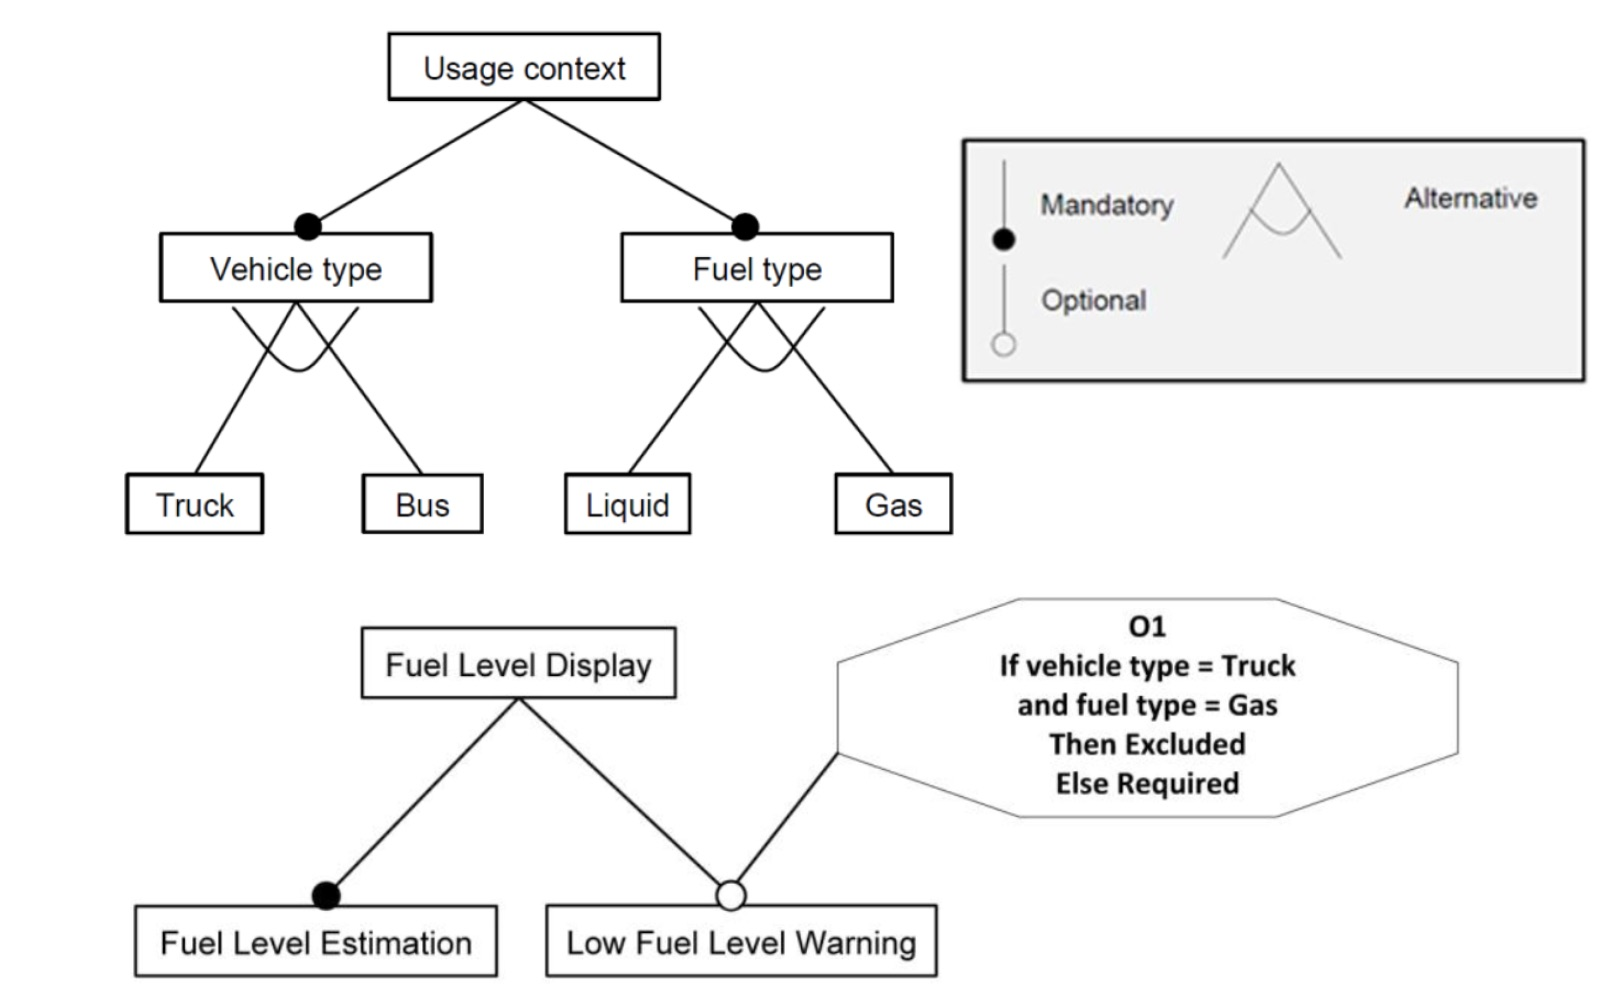
\includegraphics[width=0.75\textwidth]{FeatureDiagram}
  \caption{Feature Diagram of the FLDPL}
  \label{fig:FeatureDiagram}
\end{figure}

For example, figure \ref{fig:FeatureDiagram} shows a feature diagram of the FLDPL. In this diagram, the usage context is composed of two mandatory features: Vehicle type and Fuel type. Vehicle type can be either Truck or Bus (mutually exclusive options). Similarly, Fuel type can be either Liquid or Gas. In addition, the FLD system has one mandatory feature (Fuel Level Estimation) and one optional feature (Low Fuel Level Warning). An annotation (O1) is added to the diagram to specify the set of products where the low fuel level warning feature is present.

\subsection{Presence Condition}

\begin{description}

\item[Presence Condition]
A Presence Condition (PC) is a boolean formula over the set of features that represents the set of products in which an artifact exists.
\end{description}

For example, the presence condition for the Low Fuel Level Warning feature is: 

$\neg ($ Truck $\wedge$ Gas $)$

\subsection{Product Configuration}

\begin{description}

\item[Product Configuration]
A product configuration is a boolean formula over the set of features of an SPL that specifies the set of features present in a product.
\end{description}

For example, the configuration of an FLD for a Truck using Gas as fuel would be (Truck $\wedge$ Gas $\wedge$ FuelLevel).

\subsection{150\% Representation}

\begin{description}

\item[150\% Representation]
The 150\% representation of an SPL is a syntactic representation with syntactic constructs belonging to all the features of the SPL. 
\end{description}

Since in the vast majority of cases all those syntactic constructs can not all coexist in a product (given feature model constraints), this representation is referred to as 150\%, as opposed to the 100\% representation of a single product.

Examples of 150\% representations can be found in section 4.

\section{SPL Engineering Approaches}

SPLs are composed of features, and those features can be represented in various ways:

\lstset{
	basicstyle=\ttfamily,
     keywordstyle=\color{blue}\ttfamily,
     stringstyle=\color{red}\ttfamily,
     commentstyle=\color{green}\ttfamily,
     morecomment=[l][\color{magenta}]{\#},
	numbers=left, 
	tabsize=2,
	captionpos=b, 
	frame=shadowbox
}

\subsection{Generative}

In Generative Product Lines, each feature is designed and implemented separately, and then given a product configuration, a product is automatically generated out of the separate feature artifacts. Examples of Generative Product Line approaches include Feature-Oriented Programming \cite{Prehofer1997} and Aspect-Oriented Programming \cite{Kiczales1997}.

\begin{lstlisting}[language=Java, caption=Generative FLDPL, label={lst:Generative}, float]
// Feature module FLDGas
class FLD {
	void reportFuelLevel(float level) { 
		dashboard.display(level); 
	}
}

// Feature module FLDLiquidTruck
class FLD {
	void reportFuelLevel(float level) { 
		dashboard.display(filterKalman(level)); 
	}
}

// Feature module FLDLiquidBus
class FLD {
	void reportFuelLevel(float level) { 
		dashboard.display(filterLowPass(level)); 
	}
}

// Feature module LowGasWarning
refines class FLD {
	const float THRESHOLD;

	void reportFuelLevel(float level) { 
		if (level < THRESHOLD) { dashboard.triggerWarning()); }
		Super.reportFuelLevel(level);
	}
} 
\end{lstlisting}

Listing \ref{lst:Generative} shows a Feature-Oriented high-level implementation of FLDPL. FLDGas, FLDLiquidTruck and FLDLiquidBus are three separate implementations of the Fuel Level Display module. LowGasWarning is implemented as an orthogonal feature that refines any of the 3 FLD implementations. 

\begin{lstlisting}[language=Java, caption=Generated FLD Product, label={lst:Generated}, float]
class FLD {
	const float THRESHOLD;

	void reportFuelLevel(float level) { 
		if (level < THRESHOLD) { dashboard.triggerWarning()); }
		dashboard.display(filterKalman(level);
	}
} 
\end{lstlisting}

Given the product configuration (Liquid $\wedge$ Truck $\wedge$ FuelWarning), the product in listing \ref{lst:Generated} is generated.

\subsection{Annotative}

Generative approaches are only supported by a limited set of programming languages and tools. In mainstream languages, Annotative approaches are typically used, mainly because they don't depend on syntactic support for features, or compiler/runtime support for feature composition.

In Annotative Product Lines, a single set of artifacts is maintained, and feature expressions (Presence Conditions) are used to annotate different syntactic constructs belonging to different families of products. The most commonly used Annotative technique is C Pre-Processor (CPP) macro annotations surrounding fragments of source code.

If we are to rewrite FLDPL using CPP macros, it would look like listing \ref{lst:Annotative}. A single feature implementation (e.g. LOW\_GAS\_WARNING is now scattered across the code base, and in some cases replicated. This code snippet is an example of a 150\% representation, where a product configuration (in terms of macro definitions) excludes some of the syntactic constructs, leaving only those belonging to a specific product.

\begin{lstlisting}[language=Java, caption=Annotative FLDPL, label={lst:Annotative}, float]
class FLD {
	#if defined (LOW_GAS_WARNING)
	const float THRESHOLD;
	#endif

	void reportFuelLevel(float level) {
		#if defined (LOW_GAS_WARNING)
		if (level < THRESHOLD) { dashboard.triggerWarning(); }
		#endif

		dashboard.display(
			#if defined (FLD_GAS)
			level
			#endif

			#if defined (FLD_LIQUID_TRUCK)
			filterKalman(level);
			#endif

			#if defined (FLD_LIQUID_BUS)
			filterLowPass(level);
			#endif
		);
	}
}
\end{lstlisting}

\subsection{Delta-Oriented}

In Delta-Oriented \cite{Schaefer} Product Lines, a base product (referred to as the Core Module) is fully defined, and variants (deltas) are defined in terms of their differences with respect to the base product. 

Listing \ref{lst:Delta} shows a Delta-Oriented implementation of FLDPL. The base product here is the Gas FLD. On top of that, deltas for other variants are implemented.
 
\begin{lstlisting}[caption=Delta-Oriented FLDPL, label={lst:Delta}, float]
core FLDGas {
	class FLD {
		void reportFuelLevel(float level) { 
			dashboard.display(level); 
		}
	} 
}

delta DLiquidTruck when LiquidTruck {
	modifies class FLD {
		remove reportFuelLevel;
		add void reportFuelLevel(float level) { 
			dashboard.display(filterKalman(level)); 
		}
}

delta DLiquidBus when LiquidBus {
	modifies class FLD {
		remove reportFuelLevel;
		add void reportFuelLevel(float level) { 
			dashboard.display(filterLowPass(level)); 
		}
}

delta DLowGasWarning when LowGasWarning {
	modifies class FLD {
		add const float THRESHOLD;

		remove reportFuelLevel;
		add void reportFuelLevel(float level) {
			if (level < THRESHOLD) { dashboard.triggerWarning(); }
			FLD.reportFuelLevel(level);
		}
	}
}
\end{lstlisting}

\section{Safety Cases}

A safety case is a structured argument demonstrating the safety of a system with respect to a set of identified hazards. Hazard analysis and safety case construction are typically done for individual products. Variability in SPLs naturally leads to variability in hazards and safety cases. However, standard hazard analysis and safety case techniques and notations do not accommodate for variability. 
 
\subsection{Goal Structuring Notation (GSN)}

Goal Structuring Notation \cite{Kelly} can be used to layout logical arguments connecting safety goals to pieces of evidence satisfying them. As seen in figure \ref{fig:gsn}, a safety case in GSN is typically composed of 3 kinds of artifacts:

\begin{figure}
  \centering
  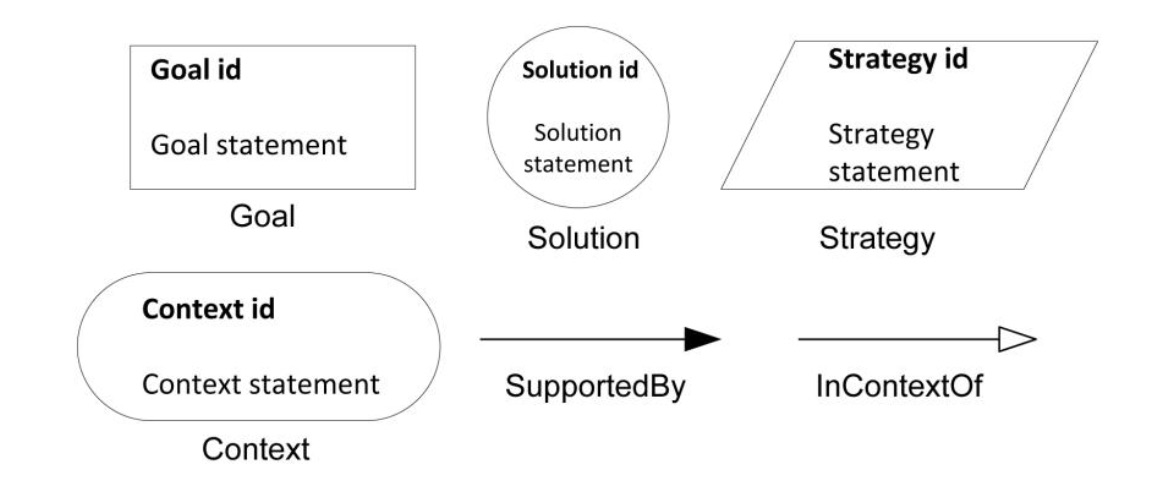
\includegraphics[width=0.75\textwidth]{gsn}
  \caption{GSN Elements}
  \label{fig:gsn}
\end{figure}

\begin{itemize}
\item Goals: These are the safety goals (requirements) identified as a result of hazard analysis techniques
\item Solutions(Evidences): These are pieces of evidence that a risk/hazard is mitigated. Evidences can be test case results, formal verification outputs, or manual investigation reports
\item Strategies: a strategy provides the logical argument connecting safety goals to their corresponding mitigating evidences
\end{itemize}

%\subsubsection{Structured Assurance Case Metamodel (SACM)}
%
%SACM \cite{SACM} is an Object Management Group (OMG) standard. SACM integrates well with other OMG metamodels (e.g. UML). It provides a much richer notation compared to GSN. The notation is composed of the following metamodels:
%
%\begin{itemize}
%\item An Argumentation Meta-model
%\item An Evidence Meta-model
%\end{itemize}
%
%\section{Adding Variability}
%
%\subsection{GSN Modules and Patterns}
%
%\subsubsection{GSN Modules}
%
%Modules are a GSN extension that facilitate modularity and reuse in safety cases. GSN elements (goals, evidences and strategies) can be packages into modules, and those modules can be reused in different contexts.
%
%\begin{figure}
%  \centering
%  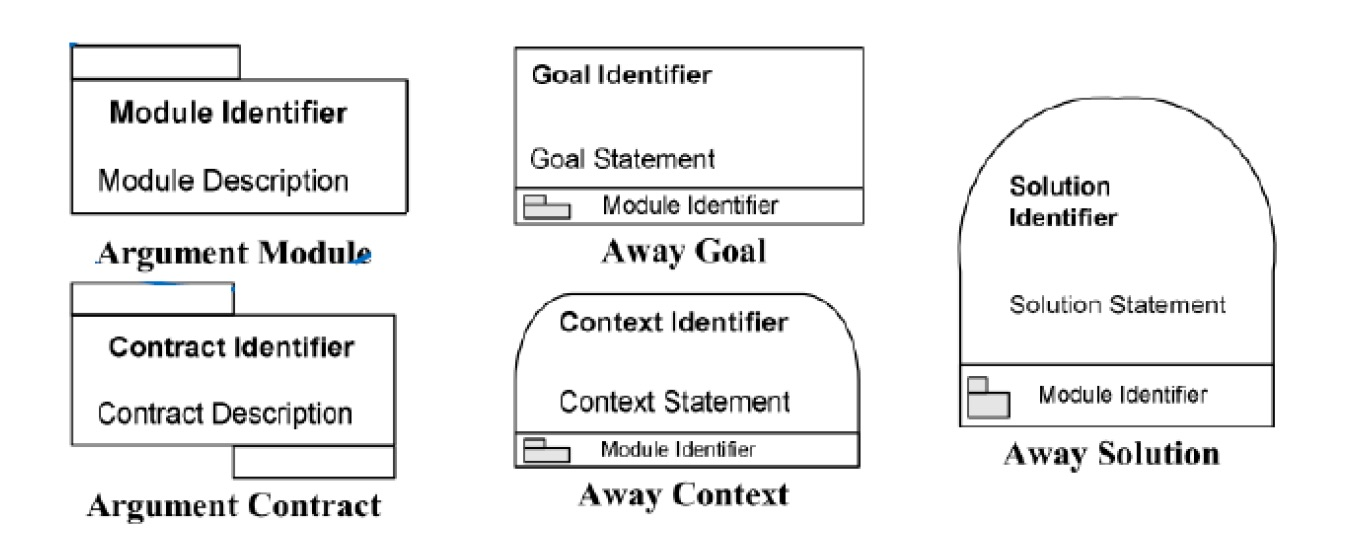
\includegraphics[width=0.75\textwidth]{gsn-modules}
%  \caption{GSN Module Constructs}
%\end{figure}
%
%\subsubsection{GSN Patterns}
%
%GSN patterns are yet another GSN extension. A GSN pattern is a parameterized GSN item. A pattern can then be instantiated by binding a parameter to a concrete value.
%
%\begin{figure}
%  \centering
%  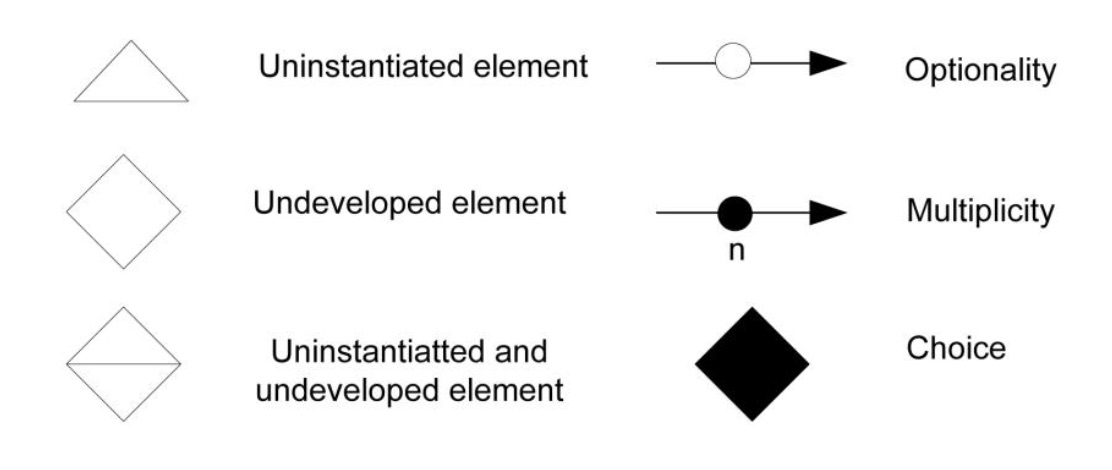
\includegraphics[width=0.75\textwidth]{gsn-patterns}
%  \caption{GSN Pattern Constructs}
%\end{figure}
%
%As an example of a GSN pattern, a generic hazard avoidance pattern would be in the context of an identified hazard, aiming at assuring that the system is safe by addressing that hazard.
%
%\begin{figure}
%  \centering
%  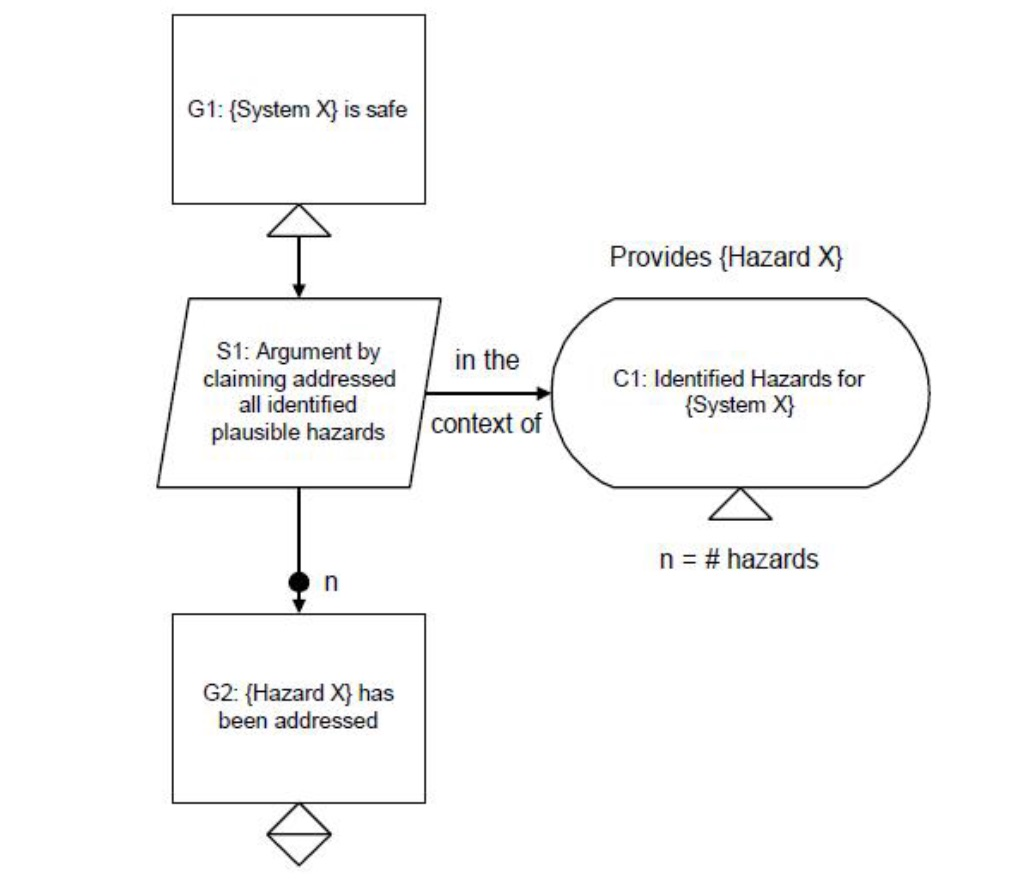
\includegraphics[width=0.75\textwidth]{gsn-pattern-example}
%  \caption{GSN Pattern Example - Hazard mitigation}
%\end{figure}
%
%\subsubsection{GSN Product Line Example}
%
%This is just a fragment of the safety case in \cite{Gallucci_2013}, demonstrating the use of GSN modules:
%
%\begin{figure}
%  \centering
%  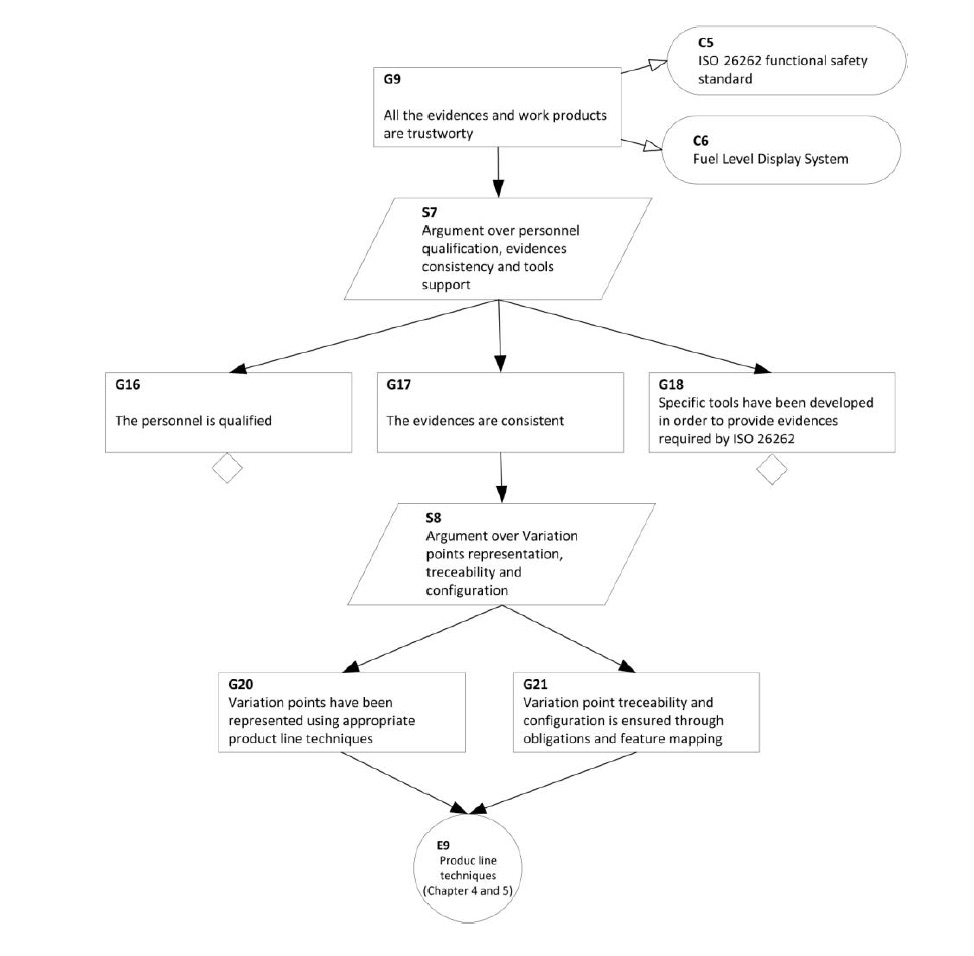
\includegraphics[width=0.75\textwidth]{safetyCase}
%  \caption{Safety Case Fragment}
%\end{figure}
%
%%3.2	Comparative Analysis
%%
%%GSN+
%%SACM?
%%GM
%%Expressivity
%%
%%
%%
%%Syntactic Conciseness
%%
%%
%%
%%Well-defined Semantics?
%%
%%
%%
%%Semantic Consistency
%%
%%
%%
%%Traceability within a single product
%%
%%
%%
%%Traceability across products
%%
%%
%%
%%
%

\subsection{Example}

For a specific Fuel Level Display (FLD) product, safety hazards are identified, and then those hazards are structurally addressed in a safety case. For example, a snippet of the FLD safety case addressing Kalman filter hazards is presented in figure \ref{fig:SafetyCaseExample}. 

Here the robustness of the estimation algorithm in the context of using the Kalman filter is a goal (G\_6). This goal is refined into a more specific goal: the steadiness of the output of the Kalman filter (G\_7).  This goal is further refined into 3 sub-goals (G\_8, G\_9, G\_10). Goal G\_8 s fulfilled by the results of standard deviation analysis (evidence E\_1). In addition, goals G\_9 and G\_10 are fulfilled by simulation results (evidence E\_2).
 
 \begin{figure}
  \centering
  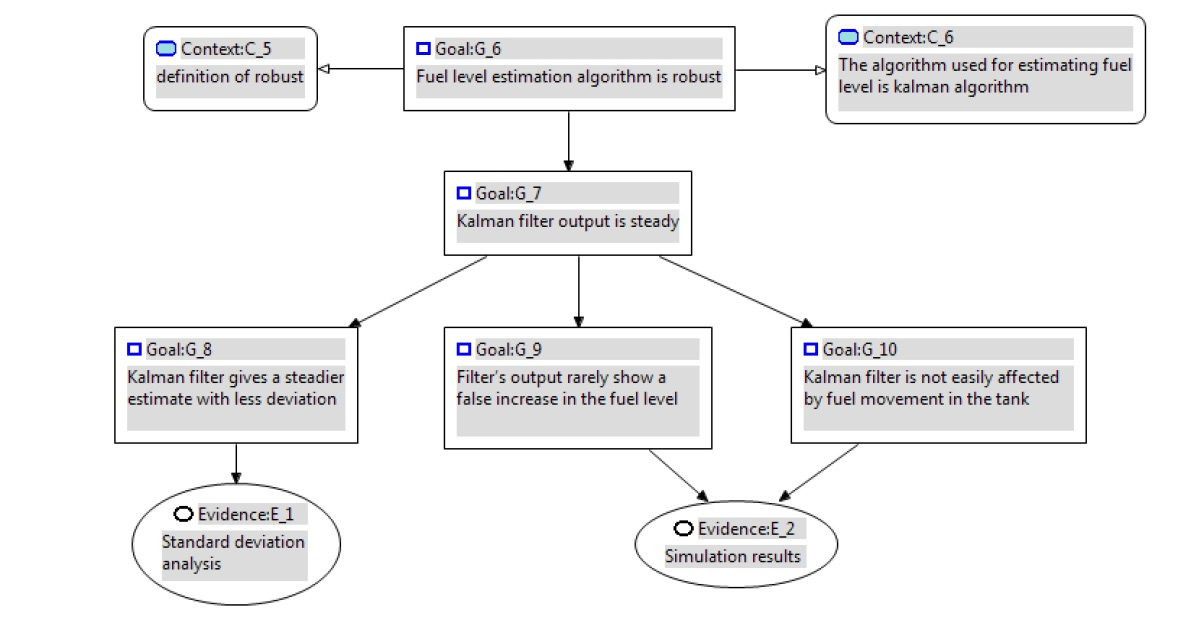
\includegraphics[width=0.75\textwidth]{SafetyCaseExample}
  \caption{Kalman filter safety case example}
  \label{fig:SafetyCaseExample}
\end{figure}

\section{Questions}

To make sure all parties agree on the context of this project, and that research work is aligned with GM practical problems, we have a few questions:

\begin{enumerate}

\item Is the example used in this document (FLDPL) representative of the SPLs developed at GM?

\item What is the product line engineering approach used by GM engineers (annotative, generative or delta-oriented)?

\item What is the safety case notation used by GM safety engineers?

\item How is safety case variability currently maintained by GM safety engineers?

\item How are hazards, safety case goals, pieces of evidence managed across different products in a product line by GM safety engineers?

\end{enumerate}
 
%\section{Product Line Engineering Scenarios}
%
%Software Product Lines can come into existence in several ways. This section briefly outline engineering scenarios for building Product Lines.
%
%\subsection{Product Evolution over Time}
%
%Starting with a single product, variability might start exhibiting itself in lots of different ways. Different deployment environments, different modes of operations, minor requirement variations from different stakeholders, and varying workloads are all examples of product-level variability. Over time, the maintenance of software artifacts with too much ad-hoc variability becomes a real problem. 
%
%One way to manage ad-hoc variability is to evolve a single product with variability in a product line. This process usually starts with factoring out a common core (common to all variants), and variant-specific artifacts.
%
%\subsection{Product Component Reuse}
%
%Again starting with a single component-oriented product, some components might be potentially reused in other products. Sometimes a component can be reused as is, without the need for any modification. In other cases the component might require minor modifications, resulting in a slightly different version. 
%
%This component-level variability can again evolve into a component-level Product Line. With more and more components being reused in this fashion, a component Product Line library becomes the skeleton of a Software Product Line.
%
%\subsection{Explicit Product-Line Engineering}
%
%The previously outlined scenarios start with a single product, and with more and more variability introduced the product evolves into a product line. Sometimes on the other hand the designers of a system are aware from day one that they are building a family or products, not just one. If at design time they draw a clear boundary between a common core and a set of varying artifacts, they are actually engineering a Product Line.
%
%\subsection{Product Lines and Safety Cases}
%
%Reasoning about Software Product Lines is not straightforward because of several reasons:
%
%\begin{itemize}
%
%\item The number of possible valid products of a product lines grows exponentially with the number of features. As a result, enumerating all possible valid products becomes intractable, and thus existing product-level reasoning techniques don't directly scale to product lines.
%
%\item A Feature Model is an integral part of a Product Line, and its role is to define the valid set of feature combinations. When reasoning about a Product Line, the Feature Model has to be taken into consideration to avoid including invalid products in any argument.
%
%\item Whenever an argument is made regarding a Product Line, it is essential to specify whether this argument applies to all valid products (universal quantification over products), or only to some (existential quantification). 
%
%\end{itemize}
%
%\subsection{Q1: Product-Line of Safety Cases or a Safety Case of a Product Line}
%
%Safety Analysis is one example of reasoning about a software systems. Techniques like Hazard Analysis, Fault Tree Analysis and Safety Cases have been well studied and applied to software products. However, when it comes to Product Lines, those techniques do not directly scale due to the previously mentioned reasons. 
%
%In addition, one fundamental question pertains to the granularity to which Safety Analysis is performed. We can think of 2 different approaches here:
%
%\begin{itemize}
%
%\item A Safety Case of a Product Line: here safety analysis as a process is applied to a Software Product Line, resulting in a single Safety Case covering the whole Product Line.
%
%\item A Product Line of Safety Cases: since a Safety Case itself is a Software Artifact (albeit a semi-formal one at best), we can have a Product Line of Safety Cases (pretty much like Product Lines of Use Case Diagrams, Class Diagrams or Source Code artifacts). 
%
%\end{itemize}
%
%\subsection{Product Line evolution impact analysis}
%
%As an SPL evolves over time (with changing requirements or more variability), existing safety cases need to evolve as well. This is essential to maintain the validity of the safety arguments. However, the safety assurance process is expensive in terms of resources and is also time consuming and labor intensive. As a result, as much of existing evidences should be reused as possible, without jeopardizing the validity of the safety arguments. Two questions are relevant here:
%
%\begin{itemize}
%
%\item Q2: As an SPL evolves, how can we determine which pieces of evidence are still valid, and can be reused as is, as opposed to pieces of evidence that are invalidated by the SPL changes?
%
%\item Q3: Within a single piece of evidence, how much reuse can be achieved? For example, if the results of a test suite and considered a piece of evidence, how much of the test cases are common across variants and how much are variant-specific? How easy is it to draw a correspondence between features, goals/sub-goals and evidences/sub-evidences? 
%
%\end{itemize}

\bibliographystyle{abbrv}
\bibliography{SafetyCasesPL}

\end{document} 